% Preamble
% Compile with XeLateX

\documentclass[11 pt,oneside,a4paper,titlepage]{article}
\usepackage{preamble}
\graphicspath{{PIC/}}
\usepackage{zh_CN-Adobefonts_external}

%%%%%%%%%%%%%%%%%%%%%%%%%%%%%%%%%%%%%%%%%%%%%%%%%%%%%%%%%%%%%%%%%%%%%%%%%%%%%%%%%%%%%%
\begin{document}

\sidebar{sideBarColor!25}
\simpleheader{appliedBlue}{彥翔}{林}{2024 英國伯明翰大學碩士應屆畢業生|多益:955|雅思學術:7|歐盟航空安全總署 Part-147 核准證書}{white}

% Start Minipages
\vspace*{3.49cm}
\adjustbox{valign=t}{\begin{minipage}{6.7cm}
    \vspace*{0.6cm}  
    % Picture
    \begin{center}
    \begin{tikzpicture}
        \node[
        circle,
        minimum size=\cvPictureWidth,
        path picture={
        \node at (path picture bounding box.center){
         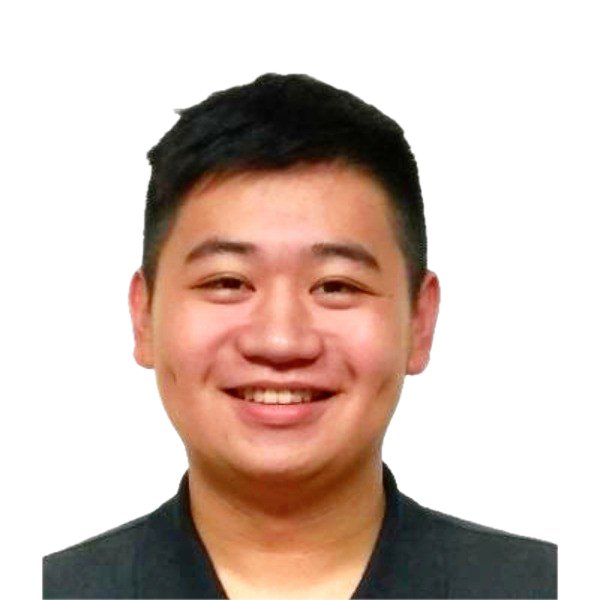
\includegraphics[width=\cvPictureWidth]{Picture.png}
         };
         }]
        {};
    \end{tikzpicture}
    \end{center}
    %%%%%%%%%%%%%%%%%%%%%%%%%%%%%%%%%%%%%%%%%%%%%%%%%%%%
    % Profile section
    \ruleline{\textbf{\color{titleBackColor} 關於我}}
    科技一直深深吸引著我,尤其是精密和先進系統的交集。
    \newline
    作為一名英國伯明翰大學的碩士應屆畢業生,我擁有高度的上進心和適應能力。我的學經歷雖然非比尋常,但卻讓我獨特地擁有了結合精準、嚴謹技術和創新的多樣化技能。從複雜的飛機修護到最前沿的電腦科學,我在硬體和軟體兩方面都建立了穩固的基礎,並且我渴望將這種獨特的融合帶入半導體產業。
    %%%%%%%%%%%%%%%%%%%%%%%%%%%%%%%%%%%%%%%%%%%%%%%%%%%
    \ruleline{\textbf{\color{titleBackColor} 語言能力}}
    \begin{tikzpicture}[every node/.style={inner sep=0pt, outer sep=0pt}]
        \matrix [
        column 1/.style={anchor=center,contactIcon},
        column 2/.style={anchor=west,align=left,contactIcon},
        column sep=5pt,
        row sep=5pt] (contact) {
        \node{\flag{England.png}};
        & \node{英文 - 多益:955,雅思學術:7};\\
        \node{\flag{taiwan.png}};
        & \node{中文 - 母語};\\
        };
    \end{tikzpicture} 
    %%%%%%%%%%%%%%%%%%%%%%%%%%%%%%%%%%%%%%%%%%%%%%%%%%%
    % Contact Section
    \ruleline{\textbf{\color{titleBackColor} 聯絡資料}}
    \begin{tikzpicture}[every node/.style={inner sep=0pt, outer sep=0pt}]
        \matrix [
        column 1/.style={anchor=center,contactIcon},
        column 2/.style={anchor=west,align=left,contactIcon},
        column sep=5pt,
        row sep=5pt] (contact) {
        \node{\circled{\faAddressCard}};
         & \node{生於:1999/07/07,25歲};\\
         & \node{兵役狀態:2024/10/31 入伍;\\\hspace{1.075cm}預計 2025/02/25 退伍};\\
        \node{\circled{\faCar}};
         & \node{普通小型車, 手/自排A 類駕照};\\
        \node{\circled{\faStreetView}};
         & \node{\href{https://www.google.com/maps/place/Zhongli+District,+Taoyuan+City,+Taiwan}{\textcolor{blue}{\underline{中壢區,桃園市,台灣} \footnotesize\faIcon{external-link-alt}}}};\\
        \node{\circled{\faEnvelope}}; 
         & \node{\href{mailto:yxl1751@alumni.bham.ac.uk}{\textcolor{blue}{\underline{yxl1751@alumni.bham.ac.uk} \footnotesize\faIcon{external-link-alt}}}};\\
        \node{\circled{\faIcon{mobile-alt}}}; 
         & \node{\href{tel:+886908890707}{\textcolor{blue}{\underline{(+886) 908 890 707} \footnotesize\faIcon{external-link-alt}}}};\\
        \node{\circled{\faIcon{mobile-alt}}}; 
         & \node{\href{tel:+447593742667}{\textcolor{blue}{\underline{(+44) 7593 742667} \footnotesize\faIcon{external-link-alt}}}};\\
        \node{\circled{\faIcon{google-drive}}}; 
         & \node{\href{https://drive.google.com/drive/folders/1xFVDNNc7-WNT1f4GN07jTezT9rDATjsx?usp=share_link}{\textcolor{blue}{\underline{drive.google.com/drive/folders} \footnotesize\faIcon{external-link-alt}}}};\\
        \node{\circled{\faGithub}};
         & \node{\href{https://github.com/Ethan-YanXiang/}{\textcolor{blue}{\underline{github.com/Ethan-YanXiang} \footnotesize\faIcon{external-link-alt}}}};\\
        \node{\circled{\faLinkedin}}; 
         & \node{\href{https://linkedin.com/in/yen-hsiang-lin/}{\textcolor{blue}{\underline{linkedin.com/in/yen-hsiang-lin} \footnotesize\faIcon{external-link-alt}}}};\\
         };
    \end{tikzpicture}
    %%%%%%%%%%%%%%%%%%%%%%%%%%%%%%%%%%%%%%%%%%%%%%%%%%%%%
    % QR Code
    \ruleline{\textbf{\color{titleBackColor} 領英 QR碼}}
    % \scriptsize
    \begin{center}
        \qrcode[height=3cm]{https://linkedin.com/in/yen-hsiang-lin/} \\ %height=2.5cm
        \vspace*{0.6cm}
        掃一下 \space 發現更多 \faLinkedin \\
    \end{center}
\end{minipage}} %
\hfill 
%%%%%%%%%%%%%%%%%%%%%%%%%%%%%%%%%%%%%%%%%%%%%%%%%%%%%%%%%
%%%%% MAIN SECTION %%%%%%%%%%%%%%%%%%%%
\adjustbox{valign=t}{\begin{minipage}{13.1cm}
    \vspace*{.7cm}
    % Work Experience
    \noindent
    \section*{\colorbox{sideBarColor!40}{\begin{minipage}{0.985\textwidth}
    \centering{\textbf{{\faToolbox} 工作經歷 \vphantom{p\^{E}}}}
    \end{minipage}}}

    \MySectionNoPic{2020/09\\ \faAngleDoubleDown \\2021/05}{LTT.png}{CAA \& EASA 許可的飛機修護工程計劃}{德國漢莎航空技術訓練}{新竹,台灣}{【學徒】}
    {\begin{itemize}[label=\Large\textbullet]
        \item 事先研究並熟悉不同手冊中與指定任務相關的所有章節,視需求依據料號/件號手冊到庫房領取替換件或耗材
        \item 依照標準作業程序,將飛機頂舉並更換機輪和煞車碟盤,執行減震支柱液壓油補充及氮氣充填服務
        \item 根據結構修理手冊的規範進行蒙皮修復,包括判定損傷是否在允許範圍內以及應用補片修復
        \item 與夥伴培養默契,在時間限制下進行維修檢查,並完成測試
        \item 在完成任務後清點並清潔手工具,以及撰寫維護記錄簿
        \item 目標在於縮短飛機地面停滯時間,保證飛機空中正常運行時數
    \end{itemize}

    \begin{multicols}{3}[\textbf{核心模組:}]
    \begin{itemize}[label=\faCaretRight]
        \item M1 \space 數學
        \item M2 \space 物理
        \item M3 \space 電氣基礎
        \item M5 \space 數位技術/電子儀表系統
        \item M6 \space 材料與硬件
        \item M7 \space 維護實踐
        \item M8 \space 基礎空氣動力學
        \item M9 \space 人因
        \item M10 \space 航空法規
        \item M11A \space 航空器之空氣動力學、結構與系統
        \item M15 \space 燃氣渦輪發動機
        \item M17 \space 螺旋槳
    \end{itemize}
    \end{multicols}
    \textbf{以全班最高總平均 90.8\% 完成所有模組,並取得 EASA Part-147 核准證書。}}
    {\faHashtag\space 預防性維護,\faHashtag\space 矯正性維護,\faHashtag\space 例行性維護,\faHashtag\space 設備安裝,\faHashtag\space 有效溝通,\faHashtag\space 故障排除,\faHashtag\space 手工具}

    %%%%%%%%%%%%%%%%%%%%%%%%%%%%%%%%%%%%%%%%%%%%%%%%%%%
    % Education
    \noindent
    \section*{\colorbox{sideBarColor!40}{\begin{minipage}{0.985\textwidth}
    \centering{\textbf{{\faUserGraduate} 教育背景 \vphantom{p\^{E}}}}
    \end{minipage}}}

    \MySection{2023/09\\ \faAngleDoubleDown \\2024/09}{BirmCrest.png}{電腦科學}{伯明翰大學}{伯明翰,英國}{【碩士】}
    {\begin{itemize}[label=\Large\textbullet]
        \item 目前,我已完成所有碩士學位模組,課程期間我專注於使用 Python 和 Flask 進行全棧網路開發,研究資料結構,並探索人工智能和機器學習領域
    \end{itemize}

    \begin{multicols}{3}[\textbf{核心模組:}]
    \begin{itemize}[label=\faCaretRight]
        \item 人工智能
        \item 機械學習
        \item 全棧開發
        \item 數據結構
        \item 演算法
        \item 資料庫
        \item 面向物件導向編程
        \item 建構可用軟件
        \item 電腦系統
        \item MSc 專案
        \item MSc 論文
    \end{itemize}
    \end{multicols}
    \textbf{模組總平均:59\%;專案提案:75\%;專案答辯:60\%;論文:評分中。}}
    {\icon{Python} Python,\icon{flask} Flask,\icon{HTML5} HTML,\icon{Bootstrap} Bootstrap,\icon{CSS3} CSS,\icon{Sqlite} SQLite,\icon{Git} git,{
\includegraphics[align=c, height=9.5pt]{PIC/Ubuntu.png}} Ubuntu,\icon{latex.png} \icon{LaTeX}}

    \vspace*{0.22cm}
        
    \MySection{2017/09\\ \faAngleDoubleDown \\2022/06}{Slogo.png}{航空機械工程}{中華科技大學}{台北,台灣}{【學士】}
    {\begin{itemize}[label=\Large\textbullet]
        \item 榮獲「第七屆四分溪文學獎」散文組內部競賽佳作
    \end{itemize}

    \begin{multicols}{3}[\textbf{相關科目:}]
    \begin{itemize}[label=\faCaretRight]
        \item 飛機系統結構
        \item 飛機氣液壓學及實習
        \item 基本電學
        \item 飛機儀電系統
        \item 飛機空氣動力學
        \item 熱力學
        \item 發動機拆裝實習
        \item 飛機結構維修
        \item 航空複合材料設計與製作
        \item 飛機性能分析
        \item 噴射推進學
    \end{itemize}
    \end{multicols}
    \textbf{學年總平均:88.84\%;總班排前 5。}}
    {\icon{multimeter} 類比/數位 \space 三用電表,\icon{Excel} Excel,\icon{Word} Word,\icon{PowerPoint} PowerPoint,\icon{CATIA} CATiA,\icon{SolidWorks} SolidWorks}
\end{minipage}} %
%%%%%%%%%%%%%%%%%%%%%%%%%%%%%%%%%%%%%%%%%%%%%%%%%%%%%%%%%%%%
% Second Page
\newpage

\simpleheader{appliedBlue}{彥翔}{林}{2024 英國伯明翰大學碩士應屆畢業生|多益:955|雅思學術:7|歐盟航空安全總署 Part-147 核准證書}{white}

%%%%%%%%%%%%%%%%%%%%%%%%%%%%%%%%%%% MAIN %%%%%%%%%%%%%%%%%%%%%%%%%
% Certificates
\vspace*{3.5cm}
\adjustbox{valign=t}{\begin{minipage}{20.4cm}
    \noindent
    \section*{\colorbox{sideBarColor!40}{\begin{minipage}{0.99\textwidth}
    \centering{\textbf{{\faIcon{award}} 官方英語能力檢定、證照與特殊成就 \vphantom{p\^{E}}}}
    \end{minipage}}}

    \adjustbox{valign=t}{\begin{minipage}{2.65cm}
        \renewcommand{\arraystretch}{1.15}
        \begin{center}
        \begin{tabular}{|c|}
            \toprule
            \toprule
            \multicolumn{1}{c}{\textbf{發照日期}} \\
            \hline
            \small \bfseries 2022/11 \\
            \hline
            \small \bfseries 2022/08 \\
            \hline
            \small \bfseries 2022/08 \\
            \hline
            \small \bfseries 2021/10 \\
            \hline
            \small \bfseries 2021/05 \\
            \hline
            \small \bfseries 2019/06 \\
            \hline
            \small \bfseries 2017/01 \\
            \hline
            \small \bfseries 2016/06 \\
            \hline
            \small \bfseries 2016/04 \\
            \hline
            \small \bfseries 2015/07 \\
            \hline
            \small \bfseries 2015/01 \\
            \hline
            \small \bfseries 2014/11 \\
            \hline
            \bottomrule
            \bottomrule
        \end{tabular}
        \end{center}
    \end{minipage}}
    \hfill \vline \hfill
    \adjustbox{valign=t}{\begin{minipage}{17.35cm}
        \renewcommand{\arraystretch}{1.15}
        \begin{center}
        \begin{tabular}{|c|c|c|c|c|}
            \toprule
            \toprule
            \multicolumn{1}{c}{\textbf{名稱}} & \multicolumn{1}{c}{\textbf{資格認證}} & \multicolumn{1}{c}{\textbf{發照機構}} & \multicolumn{1}{c}{\textbf{證照編號}} & \multicolumn{1}{c}{\textbf{查看}} \\
            \hline
            \footnotesize 雅思學術 & \footnotesize 均分 7 & \footnotesize 英國文化協會 & \footnotesize 22TW007010LINY010A & \href{https://drive.google.com/file/d/1nXDe8aJb5hxtyU3Bz6tGxo5z3RKYRuo2/view?usp=share_link}{[\icon{IELTS}]} \\
            \hline
            \footnotesize 卡內基訓練成就獎 & \footnotesize 傑出表現獎 & \footnotesize 戴爾·卡內基訓練 & \footnotesize N/A & \href{https://drive.google.com/file/d/11rWBxCaGLdCuAMQStWuuI05PkGN_mQgT/view?usp=share_link}{[\icon{Carnegie}]} \\
            \hline
            \footnotesize 卡內基訓練成就獎 & \footnotesize 最佳突破獎 & \footnotesize 戴爾·卡內基訓練 & \footnotesize N/A & \href{https://drive.google.com/file/d/1OGEcxNVhySu22TICTWzOeTMXlRTQ7Xqp/view?usp=share_link}{[\icon{Carnegie}]} \\
            \hline
            \footnotesize 多益 & \footnotesize 聽力\&閱讀 955 & \footnotesize 美國教育測驗服務社 & \footnotesize 21182247 & \href{https://drive.google.com/file/d/157b8Ev5YotJvgZlN-s8du6hFkO6T2ziH/view?usp=share_link}{[\icon{ETS}]} \\
            \hline
            \footnotesize 歐盟航空安全總署 Part-147 & \footnotesize 核准證書 & \footnotesize 德國漢莎航空技術訓練 & \footnotesize DE.147.0001.817263 & \href{https://drive.google.com/file/d/1eDd0edlxPn_dFT_rs5Mgr-INlVYq8l0e/view?usp=share_link}{[\icon{lufthansa}]} \\
            \hline
            \footnotesize 專業設計人才認證合格證書 & \footnotesize Python 3 & \footnotesize TQC+ & \footnotesize 212190800001850 & \href{https://drive.google.com/file/d/1zHnapXmb_E0XeFnB52kXoipy35wty6yH/view?usp=share_link}{[\icon{TQC+}]} \\
            \hline
            \footnotesize 飛機修護技術士證 & \footnotesize 乙級 & \footnotesize 中華民國勞動部 & \footnotesize 176-000889 & \href{https://drive.google.com/file/d/199s6IyzSsOrZRi3OvnNEyZa_Th_N4nKu/view?usp=share_link}{[\icon{MoL}]} \\
            \hline
            \footnotesize 電腦輔助立體製圖技術士證 & \footnotesize 丙級 & \footnotesize 中華民國勞動部 & \footnotesize 152-041963 & \href{https://drive.google.com/file/d/12HeVnaujeDViV7bA79XYko5WEp2ab0bG/view?usp=share_link}{[\icon{MoL}]} \\
            \hline
            \footnotesize AutoCAD 國際認證 & \footnotesize ACP & \footnotesize Autodesk & \footnotesize yWN9-DwHL & \href{https://drive.google.com/file/d/1NA8yDoOSZ_6GN7g843Ktc41dAxrr1A5t/view?usp=share_link}{[\icon{Autocad}]} \\
            \hline
            \footnotesize 自行車環台認證書 & \footnotesize 全程共 1130 公里 & \footnotesize 中國青年救國團 & \footnotesize (104)178 & \href{https://drive.google.com/file/d/19ZN_1LXMhsCw6Ij_m4gks5kYfpfLI5N2/view?usp=share_link }{[\icon{CYC}]} \\
            \hline
            \footnotesize 專業設計人才認證合格證書 & \footnotesize 工程圖學及機械製圖 & \footnotesize TQC+ & \footnotesize 212150400000360 & \href{https://drive.google.com/file/d/1n7tjVwlcXuHUcUeDnj3LIUrNxoVHBNC4/view?usp=share_link}{[\icon{TQC+}]} \\
            \hline
            \footnotesize 飛機修護技術士證 & \footnotesize 丙級 & \footnotesize 中華民國勞動部 & \footnotesize 176-012255 & \href{https://drive.google.com/file/d/1FBTc7_qhQWbfNm_MiWczNjOwyQwsvzW9/view?usp=share_link}{[\icon{MoL}]} \\
            \hline
            \bottomrule
            \bottomrule
        \end{tabular}
        \end{center}
    \end{minipage}}

    \noindent
    \section*{\colorbox{sideBarColor!40}{\begin{minipage}{0.99\textwidth}
    \centering{\textbf{{\faIcon{project-diagram}} 專案 \vphantom{p\^{E}}}}
    \end{minipage}}}

    \MyProject{2024/06\\ \faAngleDoubleDown \\2024/09}{基於無監督機器學習技術開發的即時新聞話題檢測系統}{MSc 畢業提案與專案}{3cm}{\href{https://drive.google.com/file/d/18myqKsvaKqetxzsKeF3hIDJhnjtucZch/view?usp=share_link}{[\faIcon{google-drive}]}}{\textbf{指導教授:Dr. Jizheng Wan} \hspace*{11.925cm} \href{https://github.com/Ethan-YanXiang/yxl1751.git}{[\faGithub]}}
    {\begin{multicols}{2}
    \begin{itemize}[label=\Large\textbullet, left=0pt]
        \item 多來源新聞整合:使用 Python 的 BeautifulSoup 和 Requests 庫並結合 Schedule 模組進行自動化的多來源新聞抓取和處理。抓取的新聞數據被實時用於話題檢測和文章聚類,以確保能平衡地呈現每個事件
        \item 數據清理:對抓取的新聞文本進行預處理,包括移除停用詞、標點符號、電子郵件、URL,並對詞彙進行詞幹還原,以提高文本分析的準確性
        \item TF-IDF 向量化:應用 sklearn 的 TfidfVectorizer 對清理文本進行特徵擷取,將文本轉化為向量表示。這一過程通過計算每篇文章中元素的相關性,來為後續的無監督學習算法提供支持
        \item 機器學習:實現了一個基於餘弦相似度計算的單遍聚類算法,該算法動態分配新聞文章至相應的話題類別。每當抓取到新數據時,系統會將其與現有的話題進行比較,若相似度超過閾值則歸為相同話題,否則創建新的話題類別。這樣的無監督學習算法能夠在不預先定義話題數量的情況下處理新聞數據流,以進行動態話題偵測
        \item 網路架構:使用 Flask 開發後端應用程式,處理使用者請求、資料庫互動和大型語言模型的 API 整合
        \item 情感分析:應用了自然語言處理技術(NLP),對新聞文章進行情感分類,區分正面、負面和中立的報導角度,協助用戶了解新聞的情感傾向
        \item SQLite 資料庫:使用 SQLite 作為資料儲存後端。抓取到的新聞數據,包括新聞標題、URL、發布日期、摘要、情感分析結果等都會被存儲在資料庫中,並與話題聚類結果保持同步更新
        \item 數據清理和過時數據處理:定期執行清理舊新聞數據的操作,以確保資料庫的規模可控,並減少不必要的資料冗餘
    \end{itemize}
    \end{multicols}
    \textbf{此應用提供了趨勢話題洞察力和情感分析,解決了用戶在面對海量資訊時的過濾難題,並提升了新聞消費的效率與準確性。}}
    {\icon{Overleaf} Overleaf,\icon{JetBrains} PyCharm,\icon{VS_Code} VS Code,\icon{Anaconda} Anaconda,\icon{Ollama} Ollama,\icon{learn} scikit-learn,\icon{SQLAlchemy} SQLAlchemy,\icon{Figma} Figma,\icon{GitLab} GitLab,\icon{NumPy} NumPy,\icon{Jinja2} Jinja2}

    \vspace*{0.22cm}

    \MyProject{2023/10\\ \faAngleDoubleDown \\2023/12}{即時生命體徵監測系統}{MSc 課程專案}{9.44cm}{\href{https://drive.google.com/drive/folders/1zuQ8C8KEwGzVwvmDQpdOAwV1Fg-7ZRId?usp=share_link}{[\faIcon{google-drive}]}}{\textbf{指導教授:Dr. Wendy Yanez} \\}
    {在我修讀電腦科學碩士課程的第一個學期,我和我的朋友們組成了一個小組,合作進行「建立可用的軟體」模組中的一個專案。
我們應用程式的特色是關於持續監控和協助解決不斷擴大的老年人口可能造成的問題。\\
    \begin{multicols}{2}[在作業 1 中,我們被要求在需求工程中敲定我們要設計的軟體類型;在作業 2 中,我獨自負責設計狀態圖和 Git 版本控制。\\過程中學習到:]
    \begin{itemize}[label=\Large\textbullet, left=0pt]
        \item 將任務分割成不同部分的能力有助於提高整體開發效率
        \item 運用思維導圖的技巧來幫助腦力激盪,以敲定可行的解決方案;我的想法最終貢獻於項目的背景和應用範圍的部分
        \item 功能性需求和非功能性需求之間的差異,以及使用 MoSCoW 方法組織這些需求
        \item 從使用個案和情境中抽取事件流程
        \item 從理解整個流程到有條理地將我的想法整合到 StarUML 應用程式中
    \end{itemize}
    \end{multicols}
    \textbf{吸取的教訓:1.在團隊成員間公平分配責任。 2.在將個人的貢獻合併到我們專案的最終版本時,增加一致性。 3.腦力激盪和草圖可以將複雜的任務分成幾個部分,有助於建立結構良好的圖表。}}
    {\icon{staruml} StarUML,\icon{Draw.io} draw.io,\icon{Microsoft_365} Microsoft 365}

\end{minipage}}
\end{document}
